\justify
\skipspace

This is going to be more of a summary and some implementation details of my first ever experience with computer graphics and making games.

Two weeks ago, not knowing anything about computer graphics and game development, I embarked on a journey down the rabbit hole of creating one of the pioneering games of video game history, such as the OG \textit{Doom} and \textit{Wolfenstein 3D}.

I decided to create a raycasting engine in \textit{C++} using the \textit{Simple DirectMedia Layer} graphics library. And for a beginner like me, it was quite the challenge.

The whole idea of making this in a very bare-bones library and language like \textit{SDL2} and \textit{C++} was because I wanted to create something that would be truly cross-platform from the start. And by cross-platform I mean \textbf{cross-platform}. The game would run on all desktop operating systems (Linux, Windows, Apple) and all mobile operating systems (Android, iOS, Raspberry Pi, Chrome)! And of course the \textsc{PSP}. I could talk a lot about why the PSP, but I'll save that for another time.

\section*{Introduction}

Now you must be asking - "Bruh, what even is a Raycaster".

The simplest way to explain it is that it's a rendering technique to create a 3D perspective from a 2D map, what we like to call as 2.5D.

Although this is about the making of a raycasting game engine, I had to give a lot of thought on how game engines are structured in the first place.

I wanted my project to follow the \textit{Object-Oriented} design pattern as well so that it would be easy to extend and plug in components without touching a lot of code, enabling a deeper level of abstraction. I taught me a lot about inheritance and composition in C++.

\section*{The Game Engine}

I'll talk about the game architecture in this section.

The engine was written in C++ and then compiled using the \textit{CMake} build system, which enables me to go completely cross-platform.

The high level architecture of the engine looks something like this:\\[1cm]


\begin{tikzpicture}[
    node distance = 8mm and 12mm,
    start chain = A going below,
    arr/.style = {-{Triangle[length=3mm, width=6mm]}, line width= 2mm,
    draw=blue2, shorten > = 1mm, shorten <=1mm},
    base/.style = {draw, semithick, minimum height=12mm, text width=44mm,
            align=flush center},
    BC/.style args = {#1/#2/#3}{
            decorate,
            decoration={calligraphic brace, amplitude=6pt,
                    pre =moveto, pre  length=1pt,
                    post=moveto, post length=1pt,
                    raise=#1,
                    #2},% for mirroring of brace
            very thick,
            pen colour={#3} },
    M/.style = {base, fill=#1,
            tape,
            tape bend top=none, tape bend height=2mm, tape bend bottom=in and out},
    N/.style = {base, rounded corners, fill=#1}
    ]
    % main branch
    \begin{scope}[nodes={on chain=A, join=by arr},
            N/.default=blue2]
        \node [N=blue1]     {Hi};                   % A-1
        \node [N=orange1]   {Hello};    % A-2
        \node [N]   {Hola};
        \node [N]   {He};

    \end{scope}
    % nodes on the left side of the main branch
    \node [N=gray1,
        left=of A-1]     (B-1)   {ACTEURS};
    \coordinate (aux1) at ($(A-3.south west)!0.5!(A-4.north west)$);
    \node [N=gray2,
        left=of aux1]     (B-2)   {Client};

    % nodes on the right side of thr main branch
    \begin{scope}[M/.default=yellow1]
        \node [M, right=of A-2, text width=1cm] (D-1) {C++};
    \end{scope}
\end{tikzpicture}


\section*{Raycasting}

The biggest leap of faith I took for this engine was to create the raycasting logic. So, here's how raycasting actually works.

\pgfplotsset{compat=1.15}
\usetikzlibrary{arrows}
\definecolor{zzccff}{rgb}{0.6,0.8,1}
\definecolor{ffxfqq}{rgb}{1,0.4980392156862745,0}
\definecolor{xdxdff}{rgb}{0.49019607843137253,0.49019607843137253,1}
\definecolor{cqcqcq}{rgb}{0.7529411764705882,0.7529411764705882,0.7529411764705882}
\definecolor{ududff}{rgb}{0.30196078431372547,0.30196078431372547,1}

\begin{figure}[!ht]
    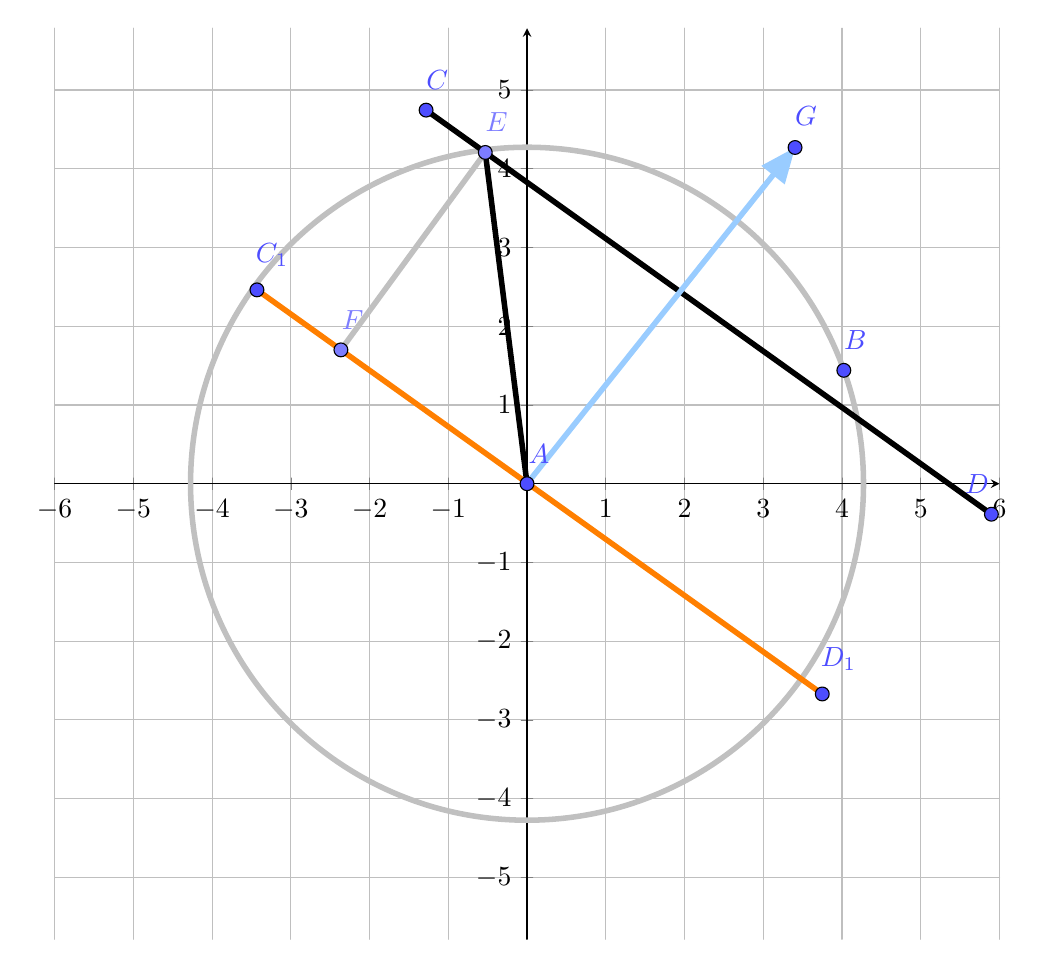
\begin{tikzpicture}[line cap=round,line join=round,>=triangle 45,x=1cm,y=1cm]
        \begin{axis}[
                x=1cm,y=1cm,
                axis lines=middle,
                ymajorgrids=true,
                xmajorgrids=true,
                xmin=-6,
                xmax=6,
                ymin=-5.784753363228701,
                ymax=5.784753363228701,
                xtick={-6,-5,...,6},
                ytick={-5,-4,...,5},]
            \clip(-6,-5.784753363228701) rectangle (6,5.784753363228701);
            \draw [line width=2pt,color=cqcqcq] (0,0) circle (4.273313221017305cm);
            \draw [line width=2pt] (-1.2820485550381981,4.744542239219644)-- (5.897465894579815,-0.38748105254433196);
            \draw [line width=2pt] (0,0)-- (-0.53013179963603,4.207061002950688);
            \draw [line width=2pt,color=ffxfqq] (-3.4299093277961026,2.4618547396848856)-- (3.7496051218219177,-2.6701685520790903);
            \draw [line width=2pt,color=cqcqcq] (-0.53013179963603,4.207061002950688)-- (-2.3636944972769713,1.699708583054546);
            \draw [->,line width=2pt,color=zzccff] (0,0) -- (3.4039247964699375,4.270028749218307);
            \begin{scriptsize}
                \draw [fill=ududff] (0,0) circle (2.5pt);
                \draw[color=ududff] (0.15246636771300448,0.3766816143497759) node {$A$};
                \draw [fill=ududff] (4.023331867972484,1.440141161511029) circle (2.5pt);
                \draw[color=ududff] (4.170403587443946,1.8295964125560542) node {$B$};
                \draw [fill=ududff] (-1.2820485550381981,4.744542239219644) circle (2.5pt);
                \draw[color=ududff] (-1.1390134529147982,5.130044843049328) node {$C$};
                \draw [fill=ududff] (5.897465894579815,-0.38748105254433196) circle (2.5pt);
                \draw[color=ududff] (5.713004484304933,0) node {$D$};
                \draw [fill=xdxdff] (-0.53013179963603,4.207061002950688) circle (2.5pt);
                \draw[color=xdxdff] (-0.38565022421524664,4.591928251121077) node {$E$};
                \draw [fill=ududff] (-3.4299093277961026,2.4618547396848856) circle (2.5pt);
                \draw[color=ududff] (-3.2376681614349776,2.9058295964125564) node {$C_{1}$};
                \draw [fill=ududff] (3.7496051218219177,-2.6701685520790903) circle (2.5pt);
                \draw[color=ududff] (3.9551569506726456,-2.224215246636772) node {$D_{1}$};
                \draw [fill=xdxdff] (-2.3636944972769713,1.699708583054546) circle (2.5pt);
                \draw[color=xdxdff] (-2.2152466367713,2.080717488789238) node {$F$};
                \draw [fill=ududff] (3.4039247964699375,4.270028749218307) circle (2.5pt);
                \draw[color=ududff] (3.5426008968609866,4.663677130044844) node {$G$};
            \end{scriptsize}
        \end{axis}
    \end{tikzpicture}
    \label{fig:circle}
\end{figure}

\newpage

